\clearpage
\subsection{Statement (Simple and Structured)} % (fold)
\label{sub:statement_with_loops_}

Statements are the actions that we can get the computer to perform.  

\begin{figure}[h]
   \centering
   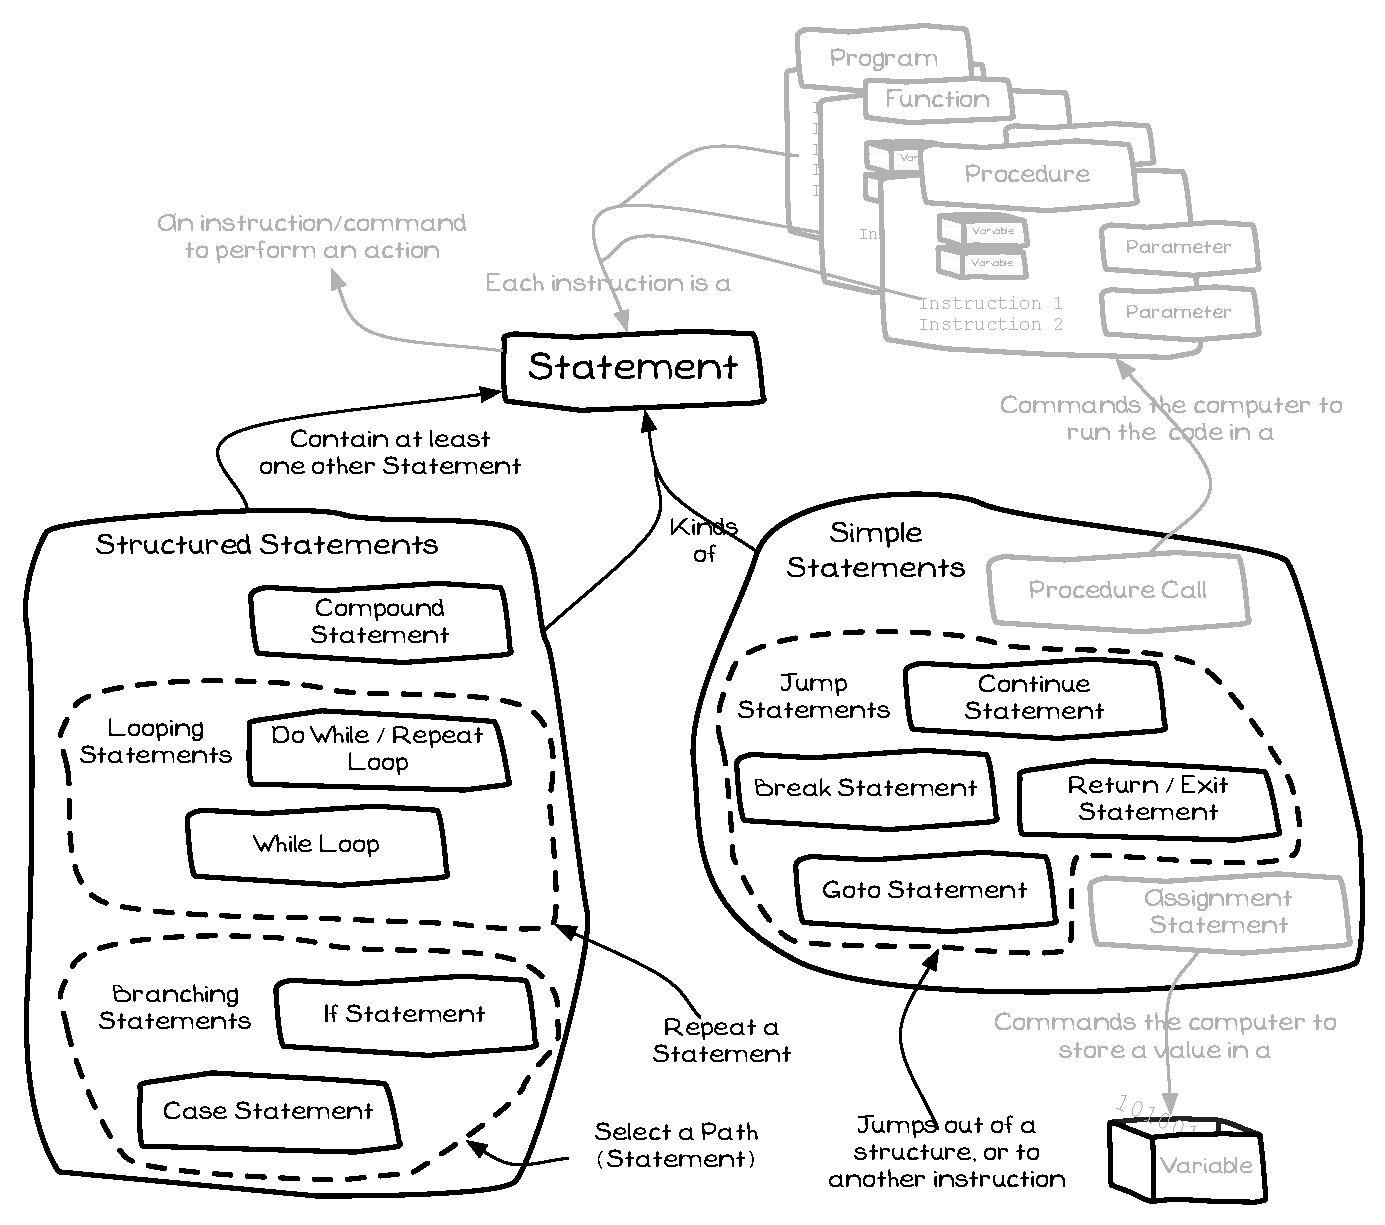
\includegraphics[width=0.88\textwidth]{./topics/control-flow/diagrams/Statement}
   \caption{A Statement may also be a Looping or Jumping Statement}
   \label{fig:looping-statement}
\end{figure}

\mynote{
\begin{itemize}
  \item Statement is the \textbf{term} given to the instructions in code.
  \item \textbf{Simple Statements} that perform an action. The actions you can perform are:
  \begin{itemize}
    \item \nameref{sub:procedure call} used to run the code in a Procedure.
    \item \nameref{sub:assignment_statement} used to calculate a value and store it in a Variable.
    \item Jump Statements allow you to affect which instruction will be performed next. This includes:
    \begin{itemize}
      \item \nameref{sub:break}: to jump out of a \nameref{sub:looping} Statement.
      \item \nameref{sub:continue}: jumps to the condition in a Looping Statement.
      \item \nameref{sub:exit}: (return in C) to end the current Function or Procedure.
      \item \nameref{sub:goto}: the unstructured jump\footnote{Often resulting in death by Raptor.} to an arbitrary location in the code.
    \end{itemize}
  \end{itemize}
  \item \textbf{Structured Statements} contain statements and control the flow of execution:
  \begin{itemize}
    \item \nameref{sub:looping} Statements: that repeat a statement a number of times.
    \begin{itemize}
      \item \nameref{sub:pre_test_loop}: Test condition before the body, repeating \textbf{0 to many} times.
      \item \nameref{sub:post_test_loop}: Test condition after the body, repeating \textbf{1 to many} times.
    \end{itemize}
    \item \nameref{sub:branching} Statement: that select from a number of optional statements.
    \begin{itemize}
      \item \nameref{sub:if_statement}: Branch based on a \nameref{sub:boolean_data} Expression (2 paths).
      \item \nameref{sub:case_statement}: Branch based on an Ordinal Expression (\emph{n} paths).
    \end{itemize}
  \end{itemize}
\end{itemize}
}


% subsection statement_with_loops_ (end)